% 问题二正文片段，可 \input 到主论文。
% 建议宏包：amsmath, amssymb, booktabs, graphicx, siunitx。

\section{基于观测几何优化的干扰源高精度定位模型}

\subsection{问题分析与模型衔接}

问题一已经在测向误差有界的条件下建立了干扰源可行区域模型。问题二不再构造新的点估计器，而是研究检测点布局如何改变多个测向角域的交会几何。其计算链为
\begin{equation}
  \text{检测点布局}\ \mathcal P
  \longrightarrow \text{问题一角域定位}
  \longrightarrow \Omega(\mathcal P)
  \longrightarrow \text{布局质量评价}.
  \label{eq:p2-chain}
\end{equation}

设第$i$个检测点为$P_i=(x_i,y_i)$，测得方向为$\theta_i$，确定性测向误差界为$\delta=1^\circ$。沿用问题一的圆周角距$d_{\mathbb S^1}$，布局$\mathcal P=\{P_1,\ldots,P_n\}$对应的可行区域为
\begin{equation}
  \Omega(\mathcal P)=B_R\cap\bigcap_{i=1}^{n}
  \left\{X\ne P_i:
  d_{\mathbb S^1}\!\left(\arg(X-P_i),\theta_i\right)\le\delta\right\},
  \qquad R=1800\ \mathrm m.
  \label{eq:p2-region}
\end{equation}
问题二程序直接调用问题一的自适应网格求解器，因而继续保留$K_{\mathrm{in}}\subseteq\overline\Omega\subseteq K_{\mathrm{out}}$的数值包络关系。有限网格点不被解释为连续区域本身。

布局规划发生在真实干扰源未知时。实际应用中，以问题一当前可行域的面积质心等代表点作为目标参考位置$\widehat S$；候选检测点围绕$\widehat S$生成。为了单独验证观测几何，本节受控实验令$\widehat S=S$，其中$S$为已知仿真真值。该处理仅用于实验控制，不代表在线任务预先知道干扰源位置。

\subsection{候选检测点与布局约束}

在$\widehat S$周围半径$r_o=1000\ \mathrm m$的圆周上，每隔$15^\circ$生成一个候选点：
\begin{equation}
  C_k=\widehat S+r_o
  \left(\cos 15k^\circ,\ \sin 15k^\circ\right),
  \qquad k=0,1,\ldots,23.
  \label{eq:p2-candidates}
\end{equation}
若候选点位于场地圆盘外则将其剔除。布局的检测点数量固定，所有点必须位于场地内；在给定选择顺序下，相邻检测点间移动距离不超过实验配置的$L_{\max}=2000\ \mathrm m$。该数值是静态布局实验的可配置工程条件，并不替代题目中的速度、总时间或障碍物规则。

图~\ref{fig:p2-layout}给出了候选点及最终六点选择顺序。
\begin{figure}[htbp]
  \centering
  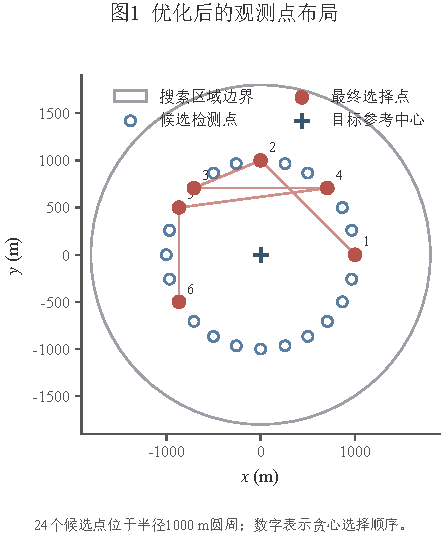
\includegraphics[width=0.56\textwidth]{../../origin_figures/Problem2_Observation_Optimization/fig01_optimized_layout.pdf}
  \caption{优化后的观测点布局}
  \label{fig:p2-layout}
\end{figure}

\subsection{布局质量指标}

以问题一得到的完整可行区域为评价对象，分别考察
\begin{equation}
  \min_{\mathcal P} A\!\left(\Omega(\mathcal P)\right),\qquad
  \min_{\mathcal P} D\!\left(\Omega(\mathcal P)\right),\qquad
  \max_{\mathcal P}\widetilde\gamma_{\min}(\mathcal P),
  \label{eq:p2-objectives}
\end{equation}
其中$A$为面积，$D$为最大区域直径。对任意两个观测方向，记原始较小夹角为$\gamma_{ij}\in[0,180^\circ]$。由于同向平行和反向共线都会造成测向线的几何退化，定义条件交会角
\begin{equation}
  \widetilde\gamma_{ij}=\min\{\gamma_{ij},180^\circ-\gamma_{ij}\},\qquad
  \widetilde\gamma_{\min}=\min_{i<j}\widetilde\gamma_{ij}.
  \label{eq:p2-conditioned-angle}
\end{equation}

面积、直径与角度具有不同量纲，若直接构造$w_1A+w_2D$，排序会依赖缺少物理依据的权重及尺度。为此，本文采用字典序评价候选点$C$：
\begin{equation}
  \operatorname{key}(C)=\left(
    A_{\mathrm{out}}(\Omega(\mathcal P\cup\{C\})),
    D_{\mathrm{out}}(\Omega(\mathcal P\cup\{C\})),
    -\widetilde\gamma_{\min},k
  \right).
  \label{eq:p2-key}
\end{equation}
首先比较问题一网格外包的面积上界；出现数值并列时，依次比较直径上界、最小条件交会角和候选编号。三个原始指标仍分别输出，不合成为单一分数。对于三站以上布局，某一对方向冗余并不意味着整个布局退化，因此$\widetilde\gamma_{\min}$仅作为解释性和破除并列的指标，不能取代$\Omega$面积。

\subsection{候选枚举与贪心选择}

算法首先用固定随机种子选择一个初始候选点。圆周候选集具有旋转对称性，初始点主要确定布局的整体方位。随后在每轮中遍历全部未选择且可达的候选点，将临时布局输入问题一，计算$A_{\mathrm{out}}$、$D_{\mathrm{out}}$和$\widetilde\gamma_{\min}$，选取式~\eqref{eq:p2-key}最小者，直到检测点数量达到要求。每轮所有候选点评价均被保存，因此选择过程可重放、可审计。

在24个候选点、最多选择6点时，除初始点外各轮最多分别评价23、22、21、20和19个候选。该方法属于可解释的局部贪心，并不声称获得组合意义下的全局最优。其核心优势是优化目标直接来自问题一的确定性可行区域，而非另行假设的点定位误差模型。

固定已有观测和测量角度时，加入新约束满足
\begin{equation}
  \Omega_{n+1}=\Omega_n\cap\Omega_{\mathrm{new}}\subseteq\Omega_n,
  \label{eq:p2-nesting}
\end{equation}
因此区域面积、直径和最小覆盖圆半径均不增加；新约束可能完全冗余，故不要求每轮严格下降。图~\ref{fig:p2-convergence}展示了零注入误差规划场景中的贪心收敛过程。

\begin{figure}[htbp]
  \centering
  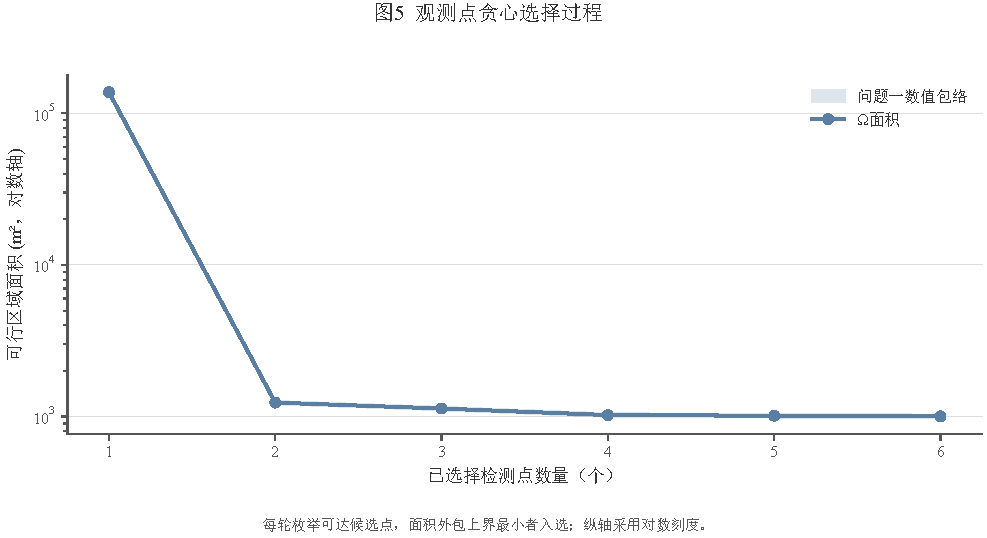
\includegraphics[width=0.88\textwidth]{../../origin_figures/Problem2_Observation_Optimization/fig05_greedy_convergence.pdf}
  \caption{观测点贪心选择过程中可行区域面积的变化}
  \label{fig:p2-convergence}
\end{figure}

\subsection{实验设计}

设置三类配对实验。第一类沿同一贪心序列依次选取前2至6个检测点，检验检测数量对区域指标的影响。第二类固定4个检测点，对比随机布局、均匀圆周布局、本文$\Omega$面积贪心布局，并额外设置DOP筛选作为诊断基线。四种布局共享候选圆、仿真真值、场景旋转和同序号测向误差。第三类固定两站到目标的距离为1000 m，将两站原始交会角$\alpha$设为30°、45°、60°、90°和120°，考察区域质心定位误差。

每个实验水平进行30次配对重复。真值在场地中心半径250 m内按面积均匀生成，测向误差在$[-1^\circ,1^\circ]$内生成。随机误差仅用于评价典型性能；问题一与问题二的定位结论仍是“误差不越界时真值属于$\Omega$”的确定性结论。均值的95\%区间由2000次百分位自举得到，该区间不是目标位置的概率置信域。

评价计算采用$200\times200$初始网格，边界精度取$0.0703\ \mathrm m$。

规划计算采用$0.2813\ \mathrm m$精度，并按面积外包上界选择候选点。
最终指标均以评价精度重算，完整参数保存在运行清单中。

\subsection{实验结果与分析}

不同布局的代表性可行区域见图~\ref{fig:p2-regions}。该样本依据预先规定的规则选取：以“优化减随机”和“优化减均匀”的面积差组成二维向量，选取标准化后最接近总体均值的重复，而非按视觉效果挑选极端样本。

\begin{figure}[htbp]
  \centering
  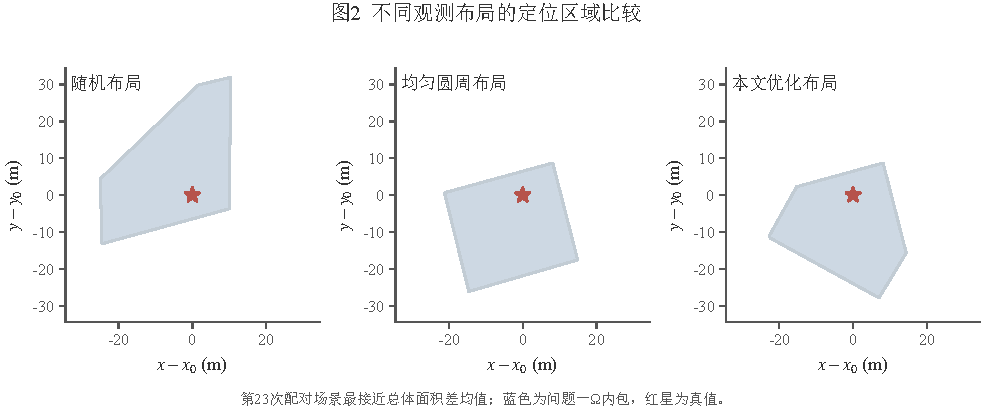
\includegraphics[width=\textwidth]{../../origin_figures/Problem2_Observation_Optimization/fig02_layout_regions.pdf}
  \caption{随机、均匀圆周与本文优化布局的可行区域比较}
  \label{fig:p2-regions}
\end{figure}

表~\ref{tab:p2-layout-comparison}表明，本文布局的平均可行区域面积为$462.886\ \mathrm{m^2}$，低于随机布局的$638.527\ \mathrm{m^2}$、均匀圆周布局的$520.174\ \mathrm{m^2}$和DOP基线的$574.535\ \mathrm{m^2}$。本文布局的平均直径同样最小，为$31.856\ \mathrm m$。但是，均匀圆周布局的平均安全覆盖半径为$16.318\ \mathrm m$，略小于本文布局的$16.453\ \mathrm m$，因此不能声称本文方法在所有指标上均最优。

相对随机布局，本文方法的配对平均面积差为$-175.641\ \mathrm{m^2}$，95\%自举区间为$[-329.210,-23.165]\ \mathrm{m^2}$，区间未跨0；均匀布局相对随机布局的面积差区间为$[-245.005,6.289]\ \mathrm{m^2}$，该样本量下不足以确认其平均面积改善。检测点数从2增加到6时，平均面积由$1230.922\ \mathrm{m^2}$降至$237.768\ \mathrm{m^2}$，420次完整实验中的数量子实验未出现超出网格上下界的反单调现象，变化趋势见图~\ref{fig:p2-number}。

\begin{figure}[htbp]
  \centering
  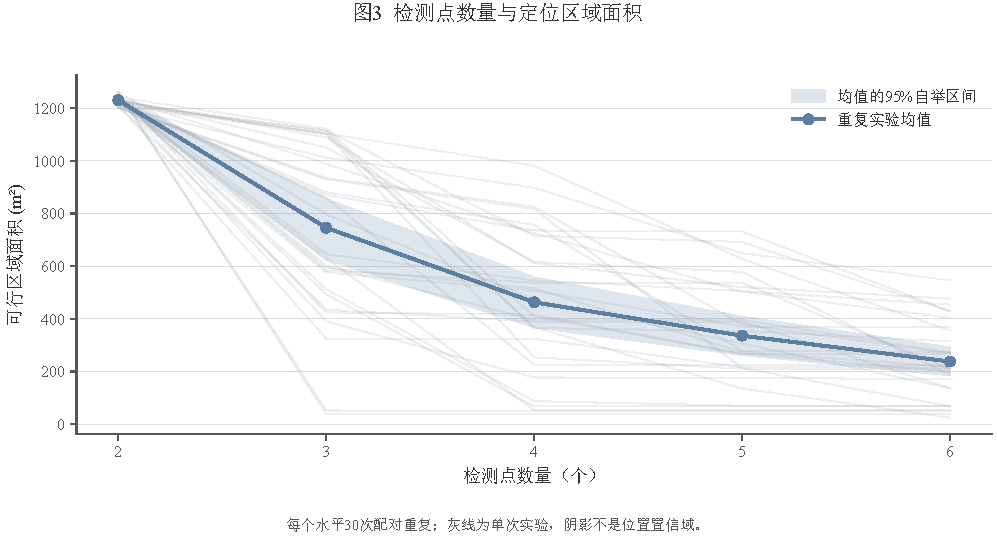
\includegraphics[width=0.88\textwidth]{../../origin_figures/Problem2_Observation_Optimization/fig03_number.pdf}
  \caption{检测点数量对可行区域面积的影响}
  \label{fig:p2-number}
\end{figure}

两站实验中，90°原始交会角的平均区域质心定位误差最低，为$14.019\ \mathrm m$；30°时增至$27.394\ \mathrm m$。60°与120°的条件角都等于60°，两者结果接近但不完全相同，原因是有限角域、测量误差实现值及场地坐标共同作用。图~\ref{fig:p2-angle}展示了完整重复轨迹和均值区间。

\begin{figure}[htbp]
  \centering
  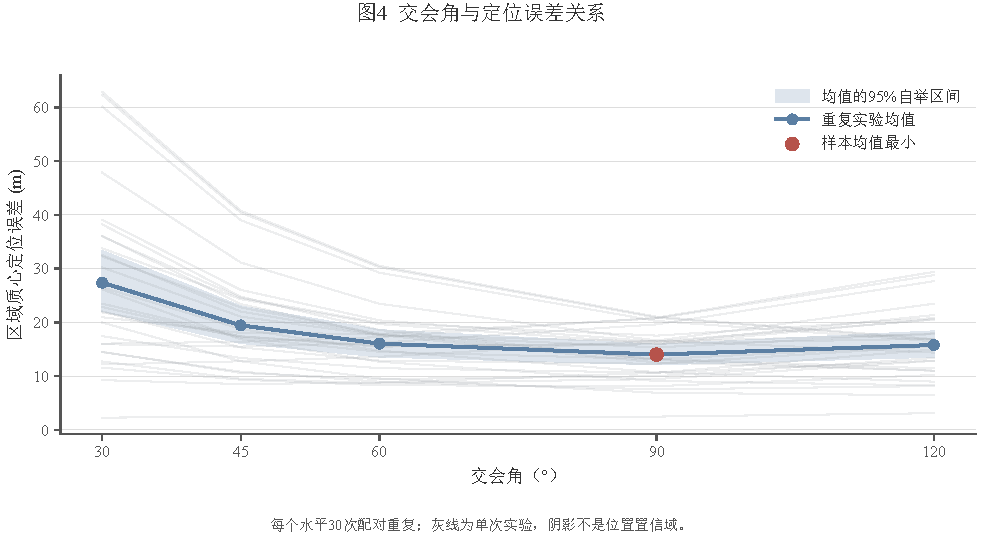
\includegraphics[width=0.88\textwidth]{../../origin_figures/Problem2_Observation_Optimization/fig04_angle.pdf}
  \caption{两站原始交会角与区域质心定位误差的关系}
  \label{fig:p2-angle}
\end{figure}

\subsection{DOP诊断与适用边界}

令$H$的每一行为观测方向的单位法向量，传统方向几何指标可写为
\begin{equation}
  \mathrm{DOP}=\sqrt{\operatorname{tr}\!\left[(H^{\mathsf T}H)^{-1}\right]}.
  \label{eq:p2-dop}
\end{equation}
DOP来源于目标附近的局部线性随机误差近似，不直接包含测向距离导致的角域横向宽度、有限场地截断和有界角误差的非线性边界。因此本文不以DOP作为最终优化目标，而只在同一候选集上构造DOP贪心基线，并继续用问题一的$\Omega$指标检验。

本实验中，本文布局相对DOP基线的配对结果支持面积改善。平均面积差为$-111.649\ \mathrm{m^2}$，95\%自举区间为$[-232.065,-0.351]\ \mathrm{m^2}$；直径、覆盖半径和定位误差的配对区间也均位于0以下。这说明在当前候选集、距离和误差界下，直接优化$\Omega$优于DOP筛选。该结论不能未经验证推广到其他候选集或噪声模型。

最后，候选圆以问题一代表中心$\widehat S$为基准。若该中心偏离真值，实际观测几何会与规划值不同。本模型尚未纳入障碍物、禁行区域、全程时间和连续路径成本；这些因素应作为运动执行层的约束处理，而不能通过改变问题一的确定性角域定位模型来补偿。

% 问题二三线表。需要 \usepackage{booktabs}、\usepackage{siunitx}。
% 数值来源：results/group_statistics.csv、paired_layout_comparisons.csv、paired_dop_comparison.csv。

\begin{table}[htbp]
  \centering
  \caption{不同观测布局的定位质量比较（30次配对重复）}
  \label{tab:p2-layout-comparison}
  \small
  \resizebox{\textwidth}{!}{%
  \begin{tabular}{lrrrrrr}
    \toprule
    布局方法 & 面积/\si{\metre\squared} & 直径/\si{\metre} & 覆盖半径/\si{\metre}
      & 定位误差/\si{\metre} & $\widetilde\gamma_{\min}$/\si{\degree} & DOP \\
    \midrule
    随机布局       & 638.527 & 47.470 & 23.941 & 11.389 & 13.0 & 1.231 \\
    均匀圆周布局   & 520.174 & 32.457 & \textbf{16.318} & 8.271 & 0.0 & 1.000 \\
    本文$\Omega$贪心布局 & \textbf{462.886} & \textbf{31.856} & 16.453 & \textbf{8.182} & 45.0 & 1.000 \\
    DOP诊断基线    & 574.535 & 34.762 & 18.111 & 10.232 & 45.0 & 1.000 \\
    \bottomrule
  \end{tabular}}

  \vspace{1mm}
  \parbox{0.96\linewidth}{\footnotesize 注：表内为30次重复的均值；面积为问题一网格内外包中点，直径为内包近似，覆盖半径为安全外包圆半径。DOP仅作诊断，不是最终优化目标。均匀圆周布局含反向共线点对，故最小条件交会角为0°，但其他独立方向仍可使整体几何良好。}
\end{table}

\begin{table}[htbp]
  \centering
  \caption{各布局相对随机布局的配对差}
  \label{tab:p2-paired-layout}
  \small
  \resizebox{\textwidth}{!}{%
  \begin{tabular}{lrrrr}
    \toprule
    布局方法 & 面积差/\si{\metre\squared} & 面积差95\%自举区间
      & 直径差/\si{\metre} & 定位误差差/\si{\metre} \\
    \midrule
    均匀圆周布局 & -118.353 & $[-245.005,\ 6.289]$ & -15.012 & -3.118 \\
    本文$\Omega$贪心布局 & -175.641 & $[-329.210,\ -23.165]$ & -15.613 & -3.207 \\
    DOP诊断基线 & -63.992 & $[-232.959,\ 94.206]$ & -12.708 & -1.157 \\
    \bottomrule
  \end{tabular}}

  \vspace{1mm}
  \parbox{0.96\linewidth}{\footnotesize 注：差值定义为“相应方法减随机布局”，负值表示指标减小。自举区间针对重复场景均值，不是干扰源位置的概率置信域。}
\end{table}

\begin{table}[htbp]
  \centering
  \caption{本文布局下检测点数量对定位质量的影响}
  \label{tab:p2-number}
  \small
  \begin{tabular}{rrrrr}
    \toprule
    检测点数$n$ & 面积/\si{\metre\squared} & 直径/\si{\metre}
      & 覆盖半径/\si{\metre} & 定位误差/\si{\metre} \\
    \midrule
    2 & 1230.922 & 49.744 & 24.969 & 14.019 \\
    3 & 746.004  & 45.130 & 22.671 & 10.921 \\
    4 & 462.886  & 31.856 & 16.453 & 8.182 \\
    5 & 336.061  & 29.684 & 15.146 & 7.577 \\
    6 & 237.768  & 25.468 & 12.963 & 5.905 \\
    \bottomrule
  \end{tabular}
\end{table}

\begin{table}[htbp]
  \centering
  \caption{两站原始交会角对区域定位结果的影响}
  \label{tab:p2-angle}
  \small
  \begin{tabular}{rrrrr}
    \toprule
    原始交会角$\alpha$/\si{\degree} & 面积/\si{\metre\squared}
      & 直径/\si{\metre} & 覆盖半径/\si{\metre} & 定位误差/\si{\metre} \\
    \midrule
    30  & 2536.352 & 138.126 & 69.255 & 27.394 \\
    45  & 1766.752 & 92.453  & 46.363 & 19.452 \\
    60  & 1432.368 & 70.418  & 35.322 & 16.056 \\
    90  & \textbf{1230.922} & \textbf{49.744} & \textbf{24.969} & \textbf{14.019} \\
    120 & 1413.802 & 69.516  & 34.881 & 15.799 \\
    \bottomrule
  \end{tabular}

  \vspace{1mm}
  \parbox{0.96\linewidth}{\footnotesize 注：此表横轴是两站原始夹角$\alpha\in[0,180^\circ]$；多站布局诊断采用$\widetilde\gamma=\min(\gamma,180^\circ-\gamma)$，故原始120°对应条件角60°。}
\end{table}

\begin{table}[htbp]
  \centering
  \caption{本文$\Omega$贪心布局与DOP基线的直接配对比较}
  \label{tab:p2-dop-direct}
  \small
  \begin{tabular}{lrr}
    \toprule
    指标（本文减DOP） & 配对均值差 & 95\%自举区间 \\
    \midrule
    面积/\si{\metre\squared} & -111.649 & $[-232.065,\ -0.351]$ \\
    直径/\si{\metre} & -2.905 & $[-5.792,\ -0.354]$ \\
    覆盖半径/\si{\metre} & -1.658 & $[-3.268,\ -0.227]$ \\
    定位误差/\si{\metre} & -2.050 & $[-3.995,\ -0.275]$ \\
    \bottomrule
  \end{tabular}
\end{table}

